% Sprint 3 — planification ch. 2 : workflow transverse (demandes, notifications, tâches, audit, chatbot)
\PFEChapterOpening{Sprint 3 - Gestion transverse des validations, notifications et traçabilité}

\section{Introduction}

Ce troisième sprint couvre les besoins transverses qui assurent la gouvernance globale de la plateforme CSR:
la soumission et le traitement des demandes de modification, la validation des plans, les notifications,
la gestion des tâches et la traçabilité des actions.

L'objectif est de fiabiliser le cycle de vie des données déjà saisies, en offrant un cadre de contrôle
cohérent entre les utilisateurs Site et Corporate.

\section{Objectif attendu}

Ce troisième sprint a pour objectif d'introduire un mécanisme de gestion globale au sein de la plateforme CSR, en structurant le cycle de validation des plans et des activités.
Il vise à encadrer les différentes étapes du cycle de validation, depuis la soumission jusqu'à la validation ou le rejet, tout en garantissant le respect des règles métier et des niveaux d'approbation définis.

Ce sprint met également en place un système de traçabilité permettant de conserver l'historique des actions effectuées, ainsi qu'un module de gestion des demandes de modification pour encadrer les ajustements après validation.
Par ailleurs, il intègre des fonctionnalités de notification et de gestion des tâches afin d'assurer une meilleure coordination entre les acteurs et un suivi efficace des actions à réaliser.

L'ensemble de ces éléments contribue à renforcer le contrôle, la transparence et la fiabilité des données, tout en assurant une gestion structurée et collaborative des processus CSR.

\section{Sprint Backlog}

Le Sprint Backlog regroupe l'ensemble des fonctionnalités retenues depuis le Product Backlog pour être développées au cours de ce sprint. Il constitue une vision détaillée et opérationnelle du travail à accomplir, en décomposant chaque fonctionnalité en tâches concrètes et réalisables.

Le tableau~\ref{tab:sprint-backlog-3} présente le backlog du troisième sprint.

% --- Sprint backlog — Workflow transverse (issu du Tableau 5.1 du brouillon Word) ---
\small
\PFETableSetup

\setlength{\PFEbacklogTabW}{\dimexpr\textwidth+2.8cm\relax}
\setlength{\LTcapwidth}{\PFEbacklogTabW}
\setlength{\LTleft}{\fill}
\setlength{\LTright}{\fill}

\setlength{\LTpre}{0pt}
\setlength{\LTpost}{0pt}

\PFETableArrayStretch
\setlength{\extrarowheight}{4pt}
\renewcommand{\arraystretch}{1.4}

\arrayrulecolor{black}

\begin{longtable}{|>{\centering\arraybackslash}m{1.2cm}|>{\raggedright\arraybackslash}m{5.2cm}|>{\centering\arraybackslash}m{1.6cm}|>{\raggedright\arraybackslash}m{5.5cm}|>{\centering\arraybackslash}m{1.7cm}|}

\caption{Sprint backlog du sprint 3 — Gestion transverse des validations, notifications et traçabilité}\label{tab:sprint-backlog-3}\\

\hline
\tableHeaderStyle
\tableHeaderCell{ID} & \tableHeaderCell{User story} & \tableHeaderCell{Tâche ID} & \tableHeaderCell{Tâche} & \tableHeaderCell{Priorité} \\
\hline
\endfirsthead

\hline
\multicolumn{5}{|c|}{\tablename\ \thetable{} — \textit{(suite)}} \\
\hline
\tableHeaderStyle
\tableHeaderCell{ID} & \tableHeaderCell{User story} & \tableHeaderCell{Tâche ID} & \tableHeaderCell{Tâche} & \tableHeaderCell{Priorité} \\
\hline
\endhead

\hline
\multicolumn{5}{|r|}{\textit{Suite page suivante\ldots}} \\
\hline
\endfoot

\hline
\endlastfoot

1 & En tant qu'utilisateur, je veux soumettre une entité (plan ou activité) afin de déclencher le processus de validation & 1.1 &
Implémenter le mécanisme de soumission (plan / activité) & +++++ \\
\cline{3-5}
& & 1.2 &
Vérifier la complétude des données avant soumission & +++++ \\
\cline{3-5}
& & 1.3 &
Changer le statut (DRAFT $\rightarrow$ SUBMITTED) & +++++ \\
\cline{3-5}
& & 1.4 &
Enregistrer la date et l'utilisateur de soumission & ++++ \\
\cline{3-5}
& & 1.5 &
Verrouiller l'entité après soumission & ++++ \\
\hline
2 & En tant qu'utilisateur Corporate, je veux valider une entité afin de confirmer sa conformité & 2.1 &
Implémenter la validation des plans et activités & +++++ \\
\cline{3-5}
& & 2.2 &
Mettre à jour le statut (Under Review $\rightarrow$ Approved) & +++++ \\
\cline{3-5}
& & 2.3 &
Enregistrer les informations de validation (date, acteur) & +++++ \\
\cline{3-5}
& & 2.4 &
Permettre la validation multi-niveaux si nécessaire & ++++ \\
\cline{3-5}
& & 2.5 &
Verrouiller l'entité validée & ++++ \\
\hline
3 & En tant qu'utilisateur Corporate, je veux rejeter une entité afin de demander une correction & 3.1 &
Implémenter le rejet des plans et activités & +++++ \\
\cline{3-5}
& & 3.2 &
Ajouter un champ commentaire obligatoire & +++++ \\
\cline{3-5}
& & 3.3 &
Mettre à jour le statut (Under Review $\rightarrow$ Rejected) & +++++ \\
\cline{3-5}
& & 3.4 &
Rendre l'entité modifiable après rejet & +++++ \\
\hline
4 & En tant qu'utilisateur Site, je veux soumettre une demande de modification afin de corriger des données verrouillées & 4.1 &
Implémenter le module de demandes de modification & +++++ \\
\cline{3-5}
& & 4.2 &
Permettre la création d'une demande avec justification et la durée & +++++ \\
\cline{3-5}
& & 4.3 &
Ajouter la gestion des pièces jointes & ++++ \\
\cline{3-5}
& & 4.4 &
Associer la demande à une entité (plan / activité) & +++++ \\
\cline{3-5}
& & 4.5 &
Définir le statut de la demande (En Attente, Approuvée, Rejetée) & ++++ \\
\hline
5 & En tant qu'utilisateur Corporate, je veux traiter les demandes de modification afin de garder le contrôle & 5.1 &
Consulter les demandes de modification & +++++ \\
\cline{3-5}
& & 5.2 &
Approuver une demande de modification & +++++ \\
\cline{3-5}
& & 5.3 &
Rejeter une demande avec justification & ++++ \\
\cline{3-5}
& & 5.4 &
Déverrouiller temporairement l'entité après approbation & ++++ \\
\hline
6 & En tant qu'utilisateur, je veux recevoir des notifications afin d'être informé des actions du système & 6.1 &
Implémenter le module de notifications & +++++ \\
\cline{3-5}
& & 6.2 &
Envoyer une notification lors de la soumission & +++++ \\
\cline{3-5}
& & 6.3 &
Envoyer une notification lors de validation & +++++ \\
\cline{3-5}
& & 6.4 &
Envoyer une notification lors de rejet & +++++ \\
\cline{3-5}
& & 6.5 &
Notifier les demandes de modification & +++++ \\
\cline{3-5}
& & 6.6 &
Permettre la consultation des notifications & ++++ \\
\hline
7 & En tant qu'utilisateur, je veux gérer mes tâches afin de suivre les actions à effectuer & 7.1 &
Implémenter le module de gestion des tâches & +++++ \\
\cline{3-5}
& & 7.2 &
Générer automatiquement une tâche après soumission & +++++ \\
\cline{3-5}
& & 7.3 &
Assigner les tâches aux utilisateurs concernés & +++++ \\
\cline{3-5}
& & 7.4 &
Permettre la consultation des tâches & ++++ \\
\hline
8 & En tant qu'utilisateur Corporate , je veux tracer toutes les actions afin d'assurer la traçabilité du système & 8.1 &
Implémenter le module d'audit & +++++ \\
\cline{3-5}
& & 8.2 &
Enregistrer chaque action (création, modification, validation\ldots) & +++++ \\
\cline{3-5}
& & 8.3 &
Associer chaque action à un utilisateur & +++++ \\
\cline{3-5}
& & 8.4 &
Enregistrer la date et le type d'action & +++++ \\
\cline{3-5}
& & 8.5 &
Permettre la consultation de l'historique & ++++ \\
\cline{3-5}
& & 8.6 &
Filtrer l'historique (par entité, action, site) & ++++ \\
\hline

\end{longtable}

\normalsize

\newpage
\section{Analyse détaillée des besoins}

\subsection{Diagramme de cas d'utilisation}

La figure~\ref{fig:doc-ch5-1} regroupe les cas d'utilisation du sprint 3 : Gestion transverse des validations, notifications et traçabilité.

\begin{figure}[H]
  \centering
  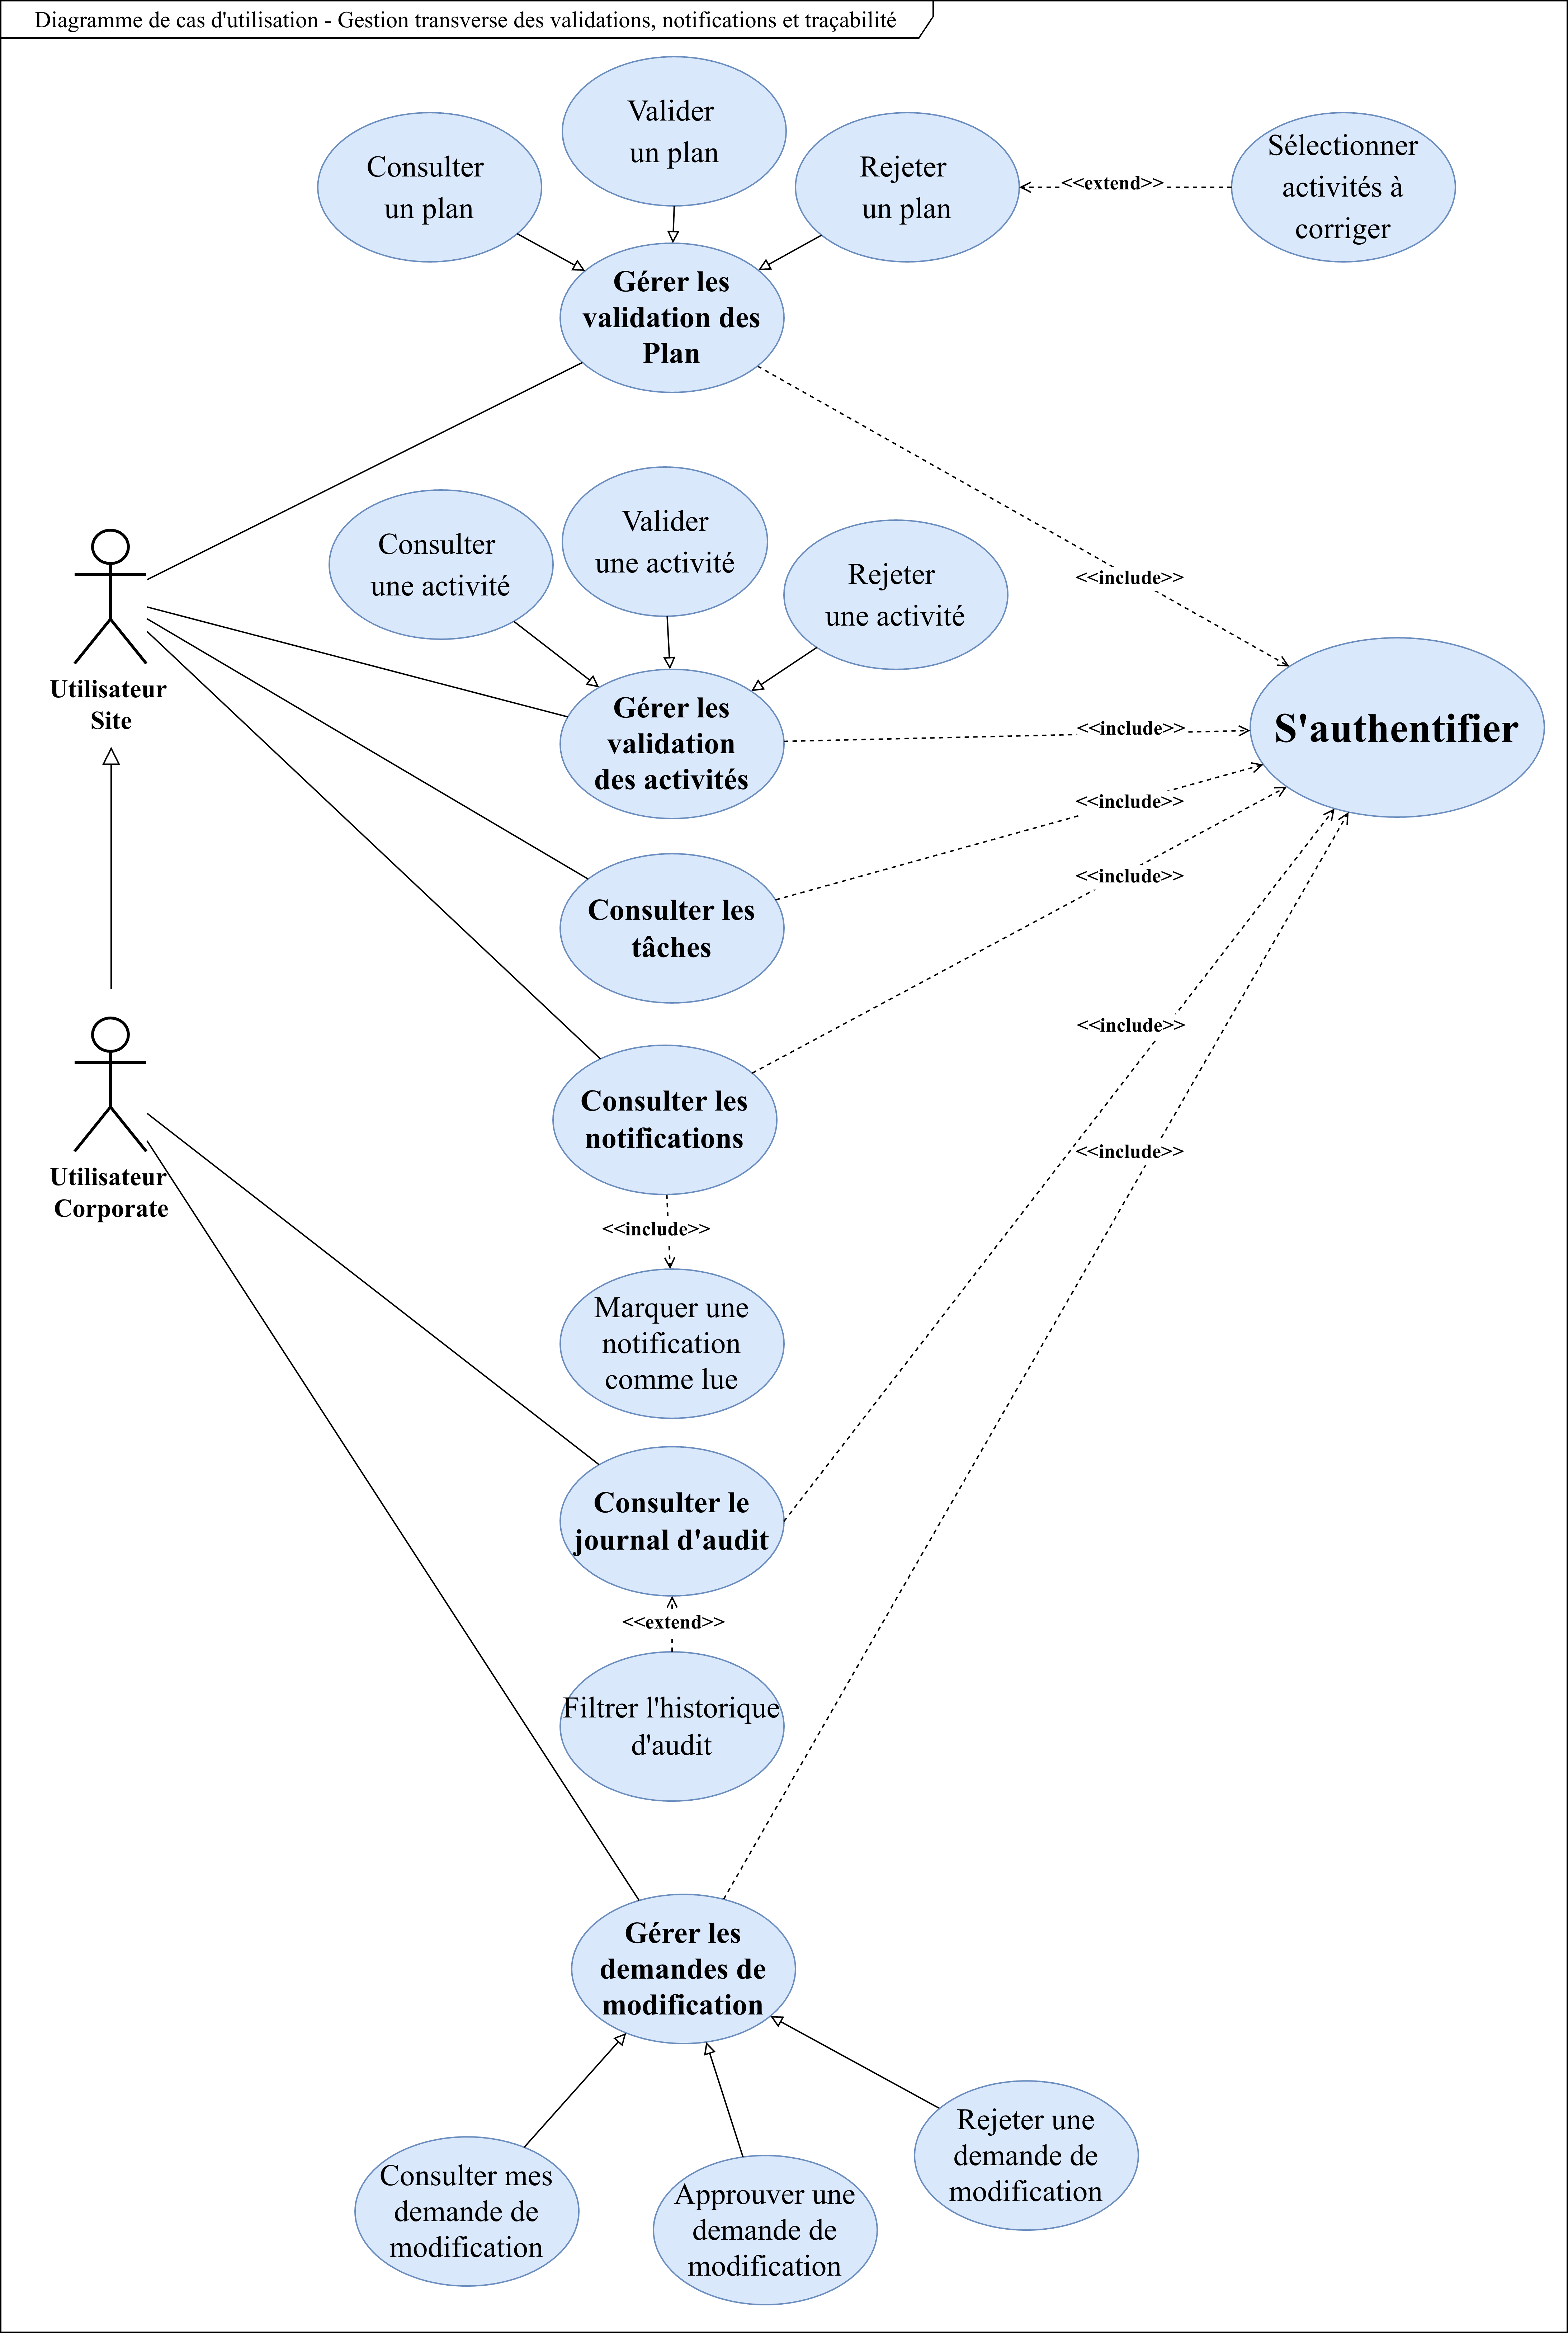
\includegraphics[width=0.85\linewidth]{figures/chapitre-05/diagramme-cas-utilisation-workflow-transverse.png}
  \caption{Diagramme de cas d'utilisation — Gestion transverse des validations, notifications et traçabilité.}
  \label{fig:doc-ch5-1}
\end{figure}%


\subsection{Description textuelle du cas d'utilisation : «~Soumettre une demande de modification pour un plan~»}

Le tableau~\ref{tab:cu-soumettre-demande-modification} expose la description textuelle du cas d'utilisation «~Soumettre une demande de modification pour un plan~».

\begin{table}[H]
  \centering
  \small
  \caption{Description textuelle du cas d'utilisation : «~Soumettre une demande de modification pour un plan~»}
  \label{tab:cu-soumettre-demande-modification}
  \PFETableSetup
  \PFETableRowColors
  \PFETableArrayStretch
  \PFETableTabularXBegin
  \begin{tabularx}{\PFETableBlockWidth}{@{}>{\raggedright\arraybackslash}p{3.2cm} >{\raggedright\arraybackslash}X@{}}
    \tableHeaderStyle
    \tableHeaderCell{Champ} & \tableHeaderCell{Contenu} \\

    \textbf{Titre} & Soumettre une demande de modification pour un plan \\

    \textbf{Acteurs} & Utilisateur Site \\

    \textbf{Objectif} &
      Permettre à l'utilisateur de formuler une demande de modification sur un plan verrouillé, afin de corriger ou ajuster des informations après validation. \\

    \textbf{Préconditions} &
      1. L'utilisateur est authentifié.\par
      2. Il est rattaché au site concerné.\par
      3. Le plan existe.\par
      4. Le plan est dans un état non modifiable. \\

    \textbf{Postconditions} &
      1. La demande de modification est enregistrée.\par
      2. Son statut est défini à «~En attente~».\par
      3. Une notification est envoyée à l'utilisateur Corporate.\par
      4. Une trace est enregistrée dans l'historique. \\

    \textbf{Scénario nominal} &
      1. L'utilisateur accède au plan concerné.\par
      2. Le système affiche les détails du plan.\par
      3. L'utilisateur sélectionne l'option de demande de modification.\par
      4. Le système affiche le formulaire de demande.\par
      5. L'utilisateur saisit les informations requises (raison, durée, ...).\par
      6. L'utilisateur joint une pièce justificative si nécessaire.\par
      7. Le système vérifie la complétude des données saisies.\par
      8. Le système enregistre la demande de modification.\par
      9. Le système déclenche une notification vers l'utilisateur Corporate.\par
      10. Le système enregistre l'action dans l'historique.\par
      11. La demande apparaît dans la liste des demandes en attente. \\

    \textbf{Scénario alternatif} &
      \textbf{1. Données incomplètes :}\par
      1.1 L'utilisateur soumet une demande avec des champs obligatoires manquants.\par
      1.2 Le système refuse la soumission.\par
      1.3 Un message d'erreur précise les informations à compléter. \\
  \end{tabularx}%
  \PFETableTabularXEnd
\end{table}


\subsection{Description textuelle du cas d'utilisation : «~Valider un plan~»}

Le tableau~\ref{tab:cu-valider-plan} expose la description textuelle du cas d'utilisation «~Valider un plan~».

\begin{table}[H]
  \centering
  \small
  \caption{Description textuelle du cas d'utilisation : «~Valider un plan~»}
  \label{tab:cu-valider-plan}
  \PFETableSetup
  \PFETableRowColors
  \PFETableArrayStretch
  \PFETableTabularXBegin
  \begin{tabularx}{\PFETableBlockWidth}{@{}>{\raggedright\arraybackslash}p{3.2cm} >{\raggedright\arraybackslash}X@{}}
    \tableHeaderStyle
    \tableHeaderCell{Champ} & \tableHeaderCell{Contenu} \\

    \textbf{Titre} & Valider un plan \\

    \textbf{Acteurs} &
      1. Utilisateur Corporate.\par
      2. Utilisateur Site (selon le mode de validation). \\

    \textbf{Objectif} &
      Permettre la validation d'un plan en respectant le circuit de validation défini, afin d'assurer la conformité et la cohérence des données avant leur exploitation. \\

    \textbf{Préconditions} &
      1. L'utilisateur est authentifié.\par
      2. Le plan  existe et est en statut «~soumis~».\par
      3. L'utilisateur dispose des droits de validation. \\

    \textbf{Postconditions} &
      1. Le statut du plan est mis à jour.\par
      2. Les informations de validation (date, acteur) sont enregistrées.\par
      3. Le plan est verrouillé après validation complète.\par
      4. Une notification est envoyée aux acteurs concernés. \\

    \textbf{Scénario nominal} &
      1. L'utilisateur accède à la liste des plans soumis.\par
      2. Le système affiche les plans en attente de validation.\par
      3. L'utilisateur sélectionne un plan et lance l'action de validation.\par
      4. Le système vérifie le mode de validation :\par
      \hspace*{1.2em}\textbf{Cas A : Mode validation directe Corporate}\par
      \hspace*{1.2em}4.1 Le système autorise la validation directe.\par
      \hspace*{1.2em}4.2 Le statut du plan passe de Soumis à validé.\par
      \hspace*{1.2em}\textbf{Cas B : Mode validation en deux étapes}\par
      \hspace*{1.2em}4.1 Le manager du site valide le plan.\par
      \hspace*{1.2em}4.2 Le plan est transmis au Corporate.\par
      \hspace*{1.2em}4.3 Le Corporate valide le plan.\par
      \hspace*{1.2em}4.4 Le statut passe à validé.\par
      5. Le système enregistre les informations de validation (acteur, date).\par
      6. Le système verrouille le plan et envoie une notification de validation. \\

    \textbf{Scénario alternatif} &
      \textbf{A. Ordre de validation non respecté :}\par
      A.1 Le Corporate tente de valider avant le manager du site.\par
      A.2 Le système refuse l'opération.\par
      A.3 Un message indique que la validation du site est requise en premier. \\
  \end{tabularx}%
  \PFETableTabularXEnd
\end{table}


\section{Modélisation conceptuelle}

\noindent
Dans cette section, nous présentons les choix de conception adoptés pour le sprint 3.
Nous commençons par le diagramme de classe, puis nous détaillons les interactions clés à travers
des diagrammes de séquence.

\subsection{Diagramme de classe}

La figure~\ref{fig:doc-ch5-2} positionne les entités liées aux demandes, notifications, validations et audit.

\begin{figure}[H]
  \centering
  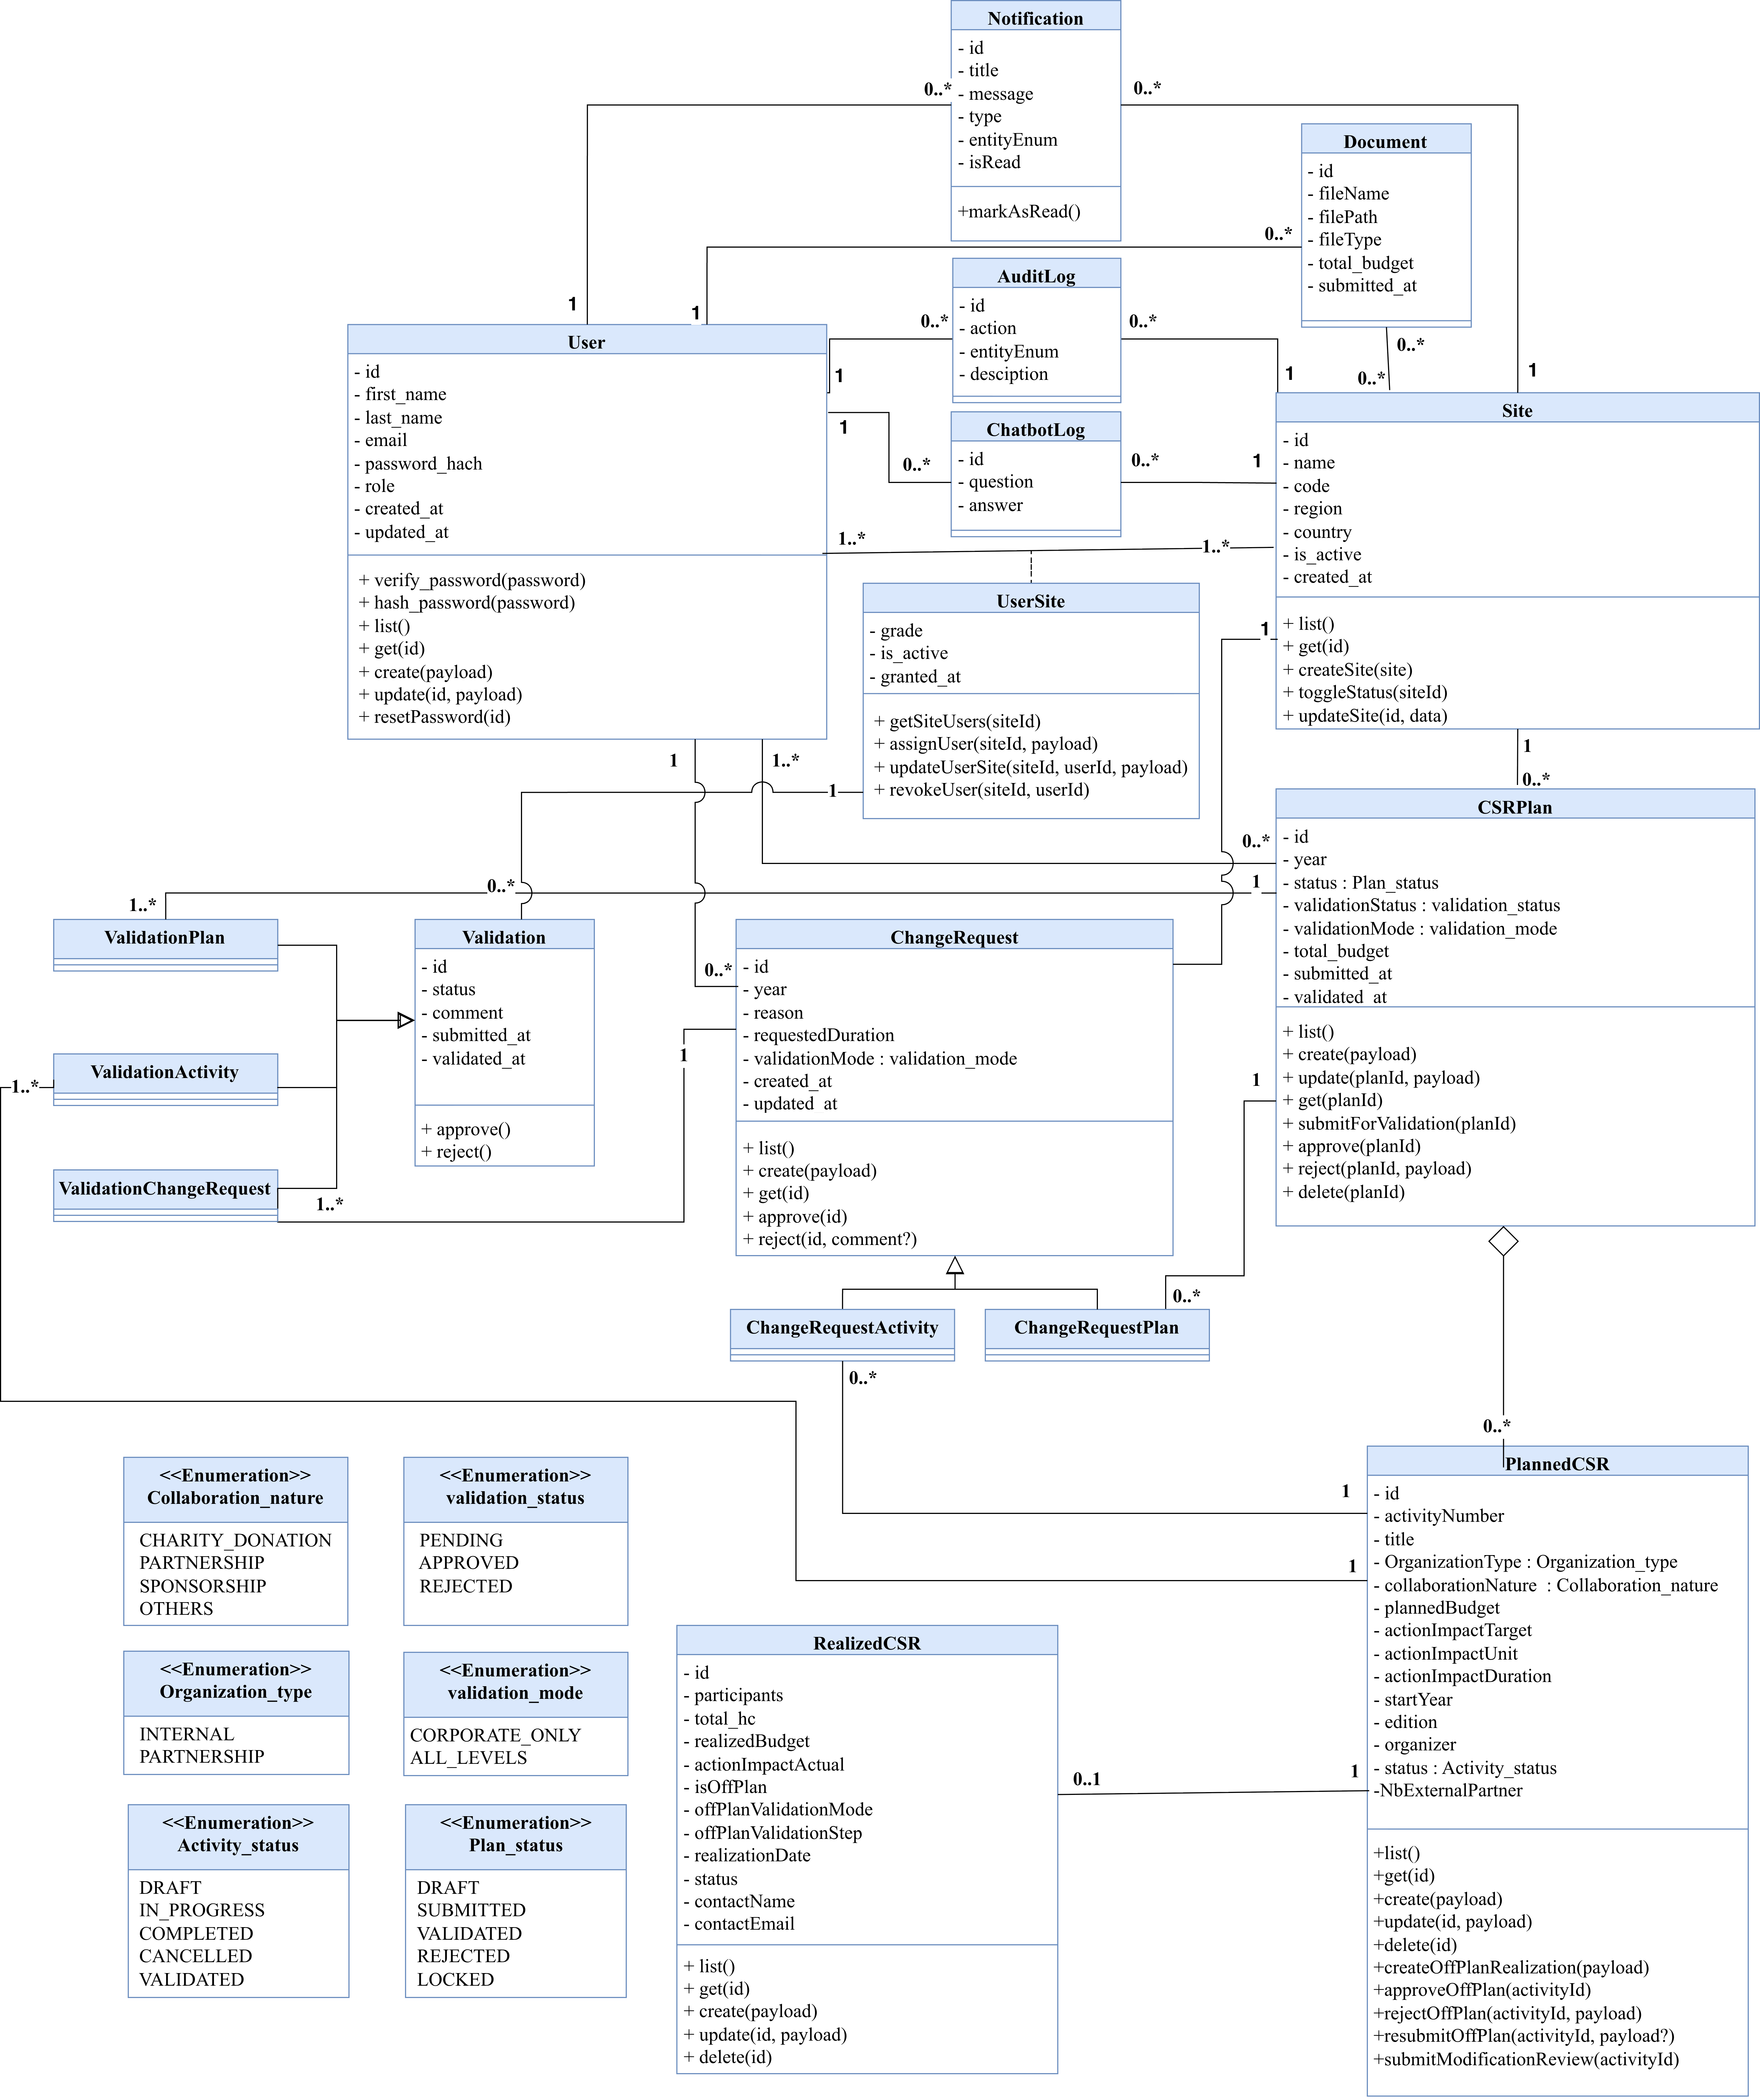
\includegraphics[width=0.92\linewidth]{figures/chapitre-05/diagramme-classe-workflow-transverse.png}
  \caption{Diagramme de classe — Gestion transverse des validations, notifications et traçabilité.}
  \label{fig:doc-ch5-2}
\end{figure}%

\subsection{Diagramme de séquence}

\subsubsection{Diagramme de séquence : «~Soumettre et traiter une demande de modification~»}

La figure~\ref{fig:doc-ch5-seq-cr} présente le scénario «~Soumettre et traiter une demande de modification~».

\IfFileExists{figures/chapitre-05/diagramme-sequence-demande-modification.png}{%
\begin{figure}[H]
  \centering
  \includegraphics[width=0.92\linewidth]{figures/chapitre-05/diagramme-sequence-demande-modification.png}
  \caption{Diagramme de séquence — demande de modification.}
  \label{fig:doc-ch5-seq-cr}
\end{figure}%
}{%
\begin{figure}[H]
  \centering
  \fbox{\parbox{0.92\linewidth}{\centering\vspace{3.2cm}\textit{(Figure à insérer : \texttt{figures/chapitre-05/diagramme-sequence-demande-modification.png})}\vspace{3.2cm}}}
  \caption{Diagramme de séquence — demande de modification.}
  \label{fig:doc-ch5-seq-cr}
\end{figure}%
}

\subsubsection{Diagramme de séquence : «~Propagation notification et tâches~»}

La figure~\ref{fig:doc-ch5-seq-notif} illustre la propagation \textbf{notification + tâche} après un événement métier.

\IfFileExists{figures/chapitre-05/diagramme-sequence-notification-tache.png}{%
\begin{figure}[H]
  \centering
  \includegraphics[width=0.92\linewidth]{figures/chapitre-05/diagramme-sequence-notification-tache.png}
  \caption{Diagramme de séquence — notification et rafraîchissement des tâches.}
  \label{fig:doc-ch5-seq-notif}
\end{figure}%
}{%
\begin{figure}[H]
  \centering
  \fbox{\parbox{0.92\linewidth}{\centering\vspace{3.2cm}\textit{(Figure à insérer : \texttt{figures/chapitre-05/diagramme-sequence-notification-tache.png})}\vspace{3.2cm}}}
  \caption{Diagramme de séquence — notification et rafraîchissement des tâches.}
  \label{fig:doc-ch5-seq-notif}
\end{figure}%
}

\section{Réalisation}

Dans cette partie, nous présentons les interfaces développées durant ce troisième sprint.
Les différentes captures illustrent les fonctionnalités mises en place, notamment le processus de validation des plans et des activités, la gestion des demandes de modification, ainsi que le suivi des notifications et des tâches.
Ces éléments permettent de visualiser concrètement le fonctionnement du workflow et de vérifier l'adéquation des fonctionnalités réalisées avec les exigences définies dans le backlog du sprint.

\subsection{Interface de validation des plans annuels}

La figure~\ref{fig:ch5-realisation-validation-plans} présente l'interface de validation des plans annuels.

\IfFileExists{figures/chapitre-05/realisation-interface-validation-plans-annuels.png}{%
\begin{figure}[H]
  \centering
  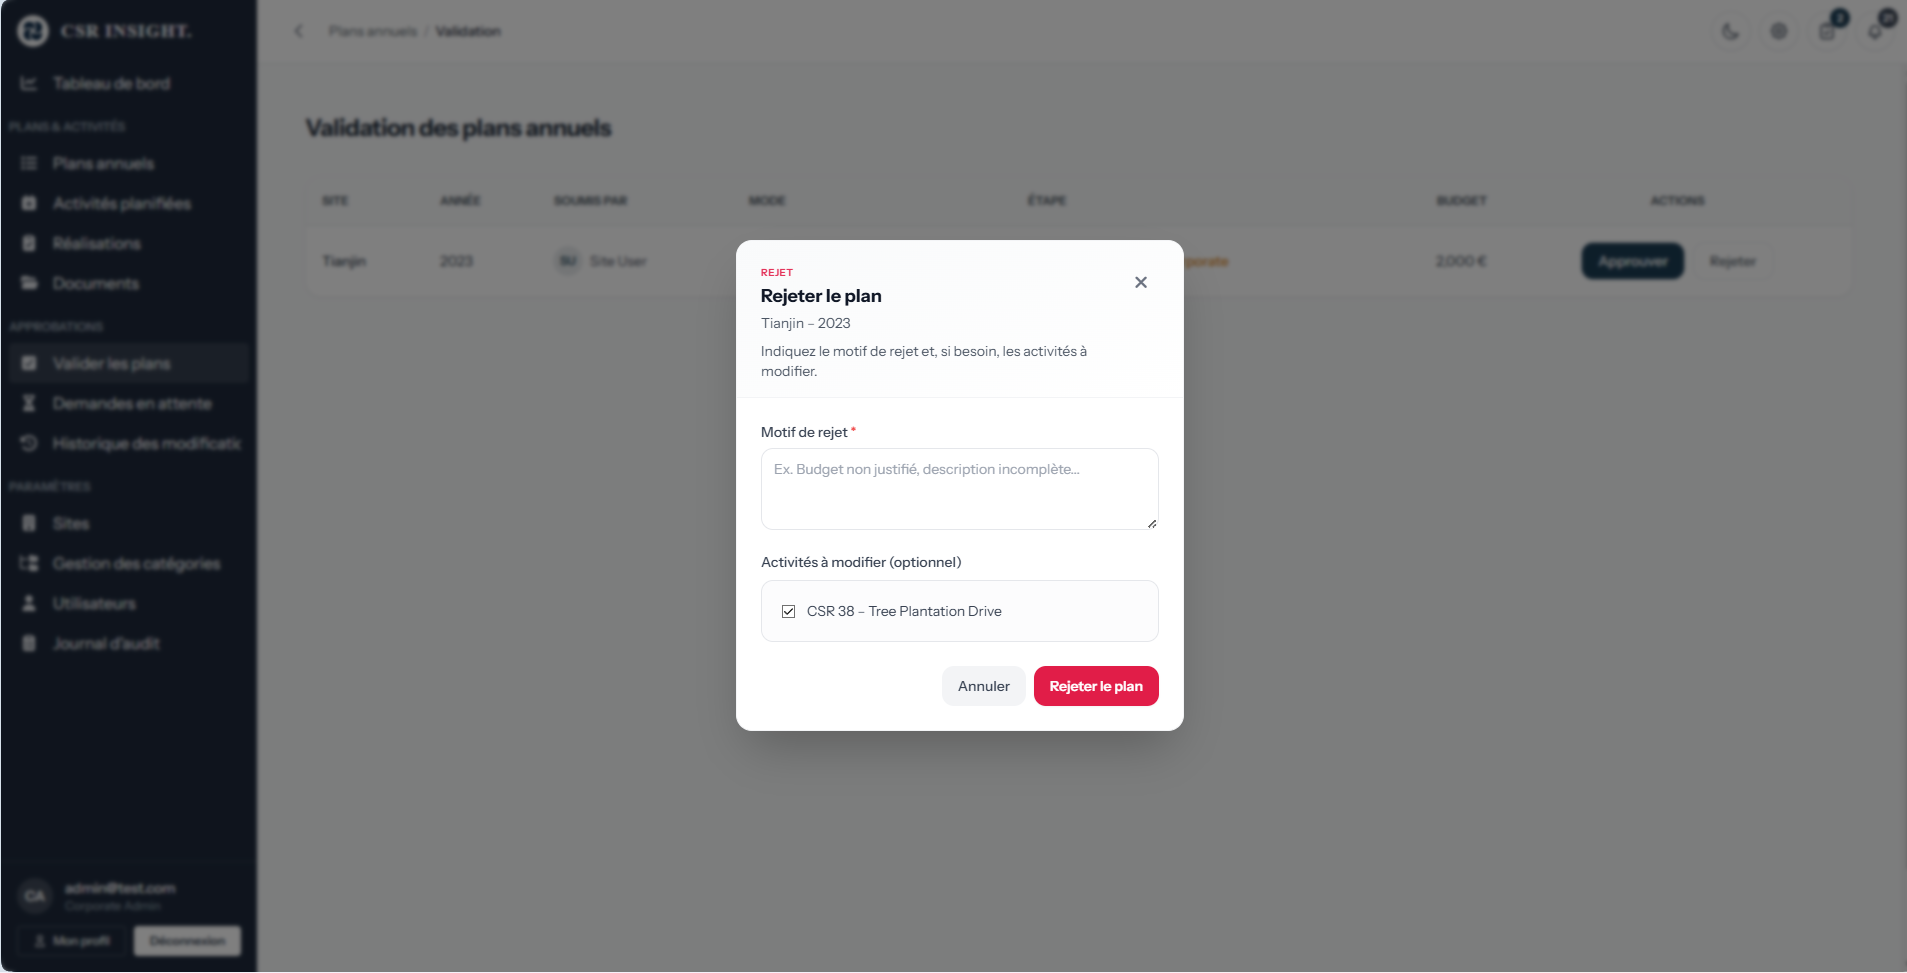
\includegraphics[width=0.92\linewidth]{figures/chapitre-05/realisation-interface-validation-plans-annuels.png}
  \caption{Interface de validation des plans annuels.}
  \label{fig:ch5-realisation-validation-plans}
\end{figure}%
}{%
\begin{figure}[H]
  \centering
  \fbox{\parbox{0.92\linewidth}{\centering\vspace{3.2cm}\textit{(Figure à insérer : \texttt{figures/chapitre-05/realisation-interface-validation-plans-annuels.png})}\vspace{3.2cm}}}
  \caption{Interface de validation des plans annuels.}
  \label{fig:ch5-realisation-validation-plans}
\end{figure}%
}

L'interface ci-dessus est dédiée à la validation des plans CSR, utilisée par l'utilisateur Corporate pour examiner les plans soumis.
Elle repose sur un tableau synthétique affichant les informations essentielles, notamment le site concerné, l'année, l'utilisateur ayant effectué la soumission, le mode de validation, l'état d'avancement ainsi que le budget associé.
Cette organisation permet d'identifier rapidement les plans en attente de décision.

Chaque ligne intègre des actions directes, telles que l'approbation ou le rejet, offrant une interaction rapide et efficace avec le système.
L'utilisateur peut ainsi traiter les demandes de validation de manière centralisée, tout en conservant une vision globale des éléments en cours.
Cette interface constitue un point clé du processus décisionnel, en facilitant le contrôle et la validation des données avant leur finalisation.

\subsection{Interface de rejet d'un plan}

La figure~\ref{fig:ch5-realisation-rejet-plan} présente l'interface de rejet d'un plan.

\IfFileExists{figures/chapitre-05/realisation-interface-rejet-plan.png}{%
\begin{figure}[H]
  \centering
  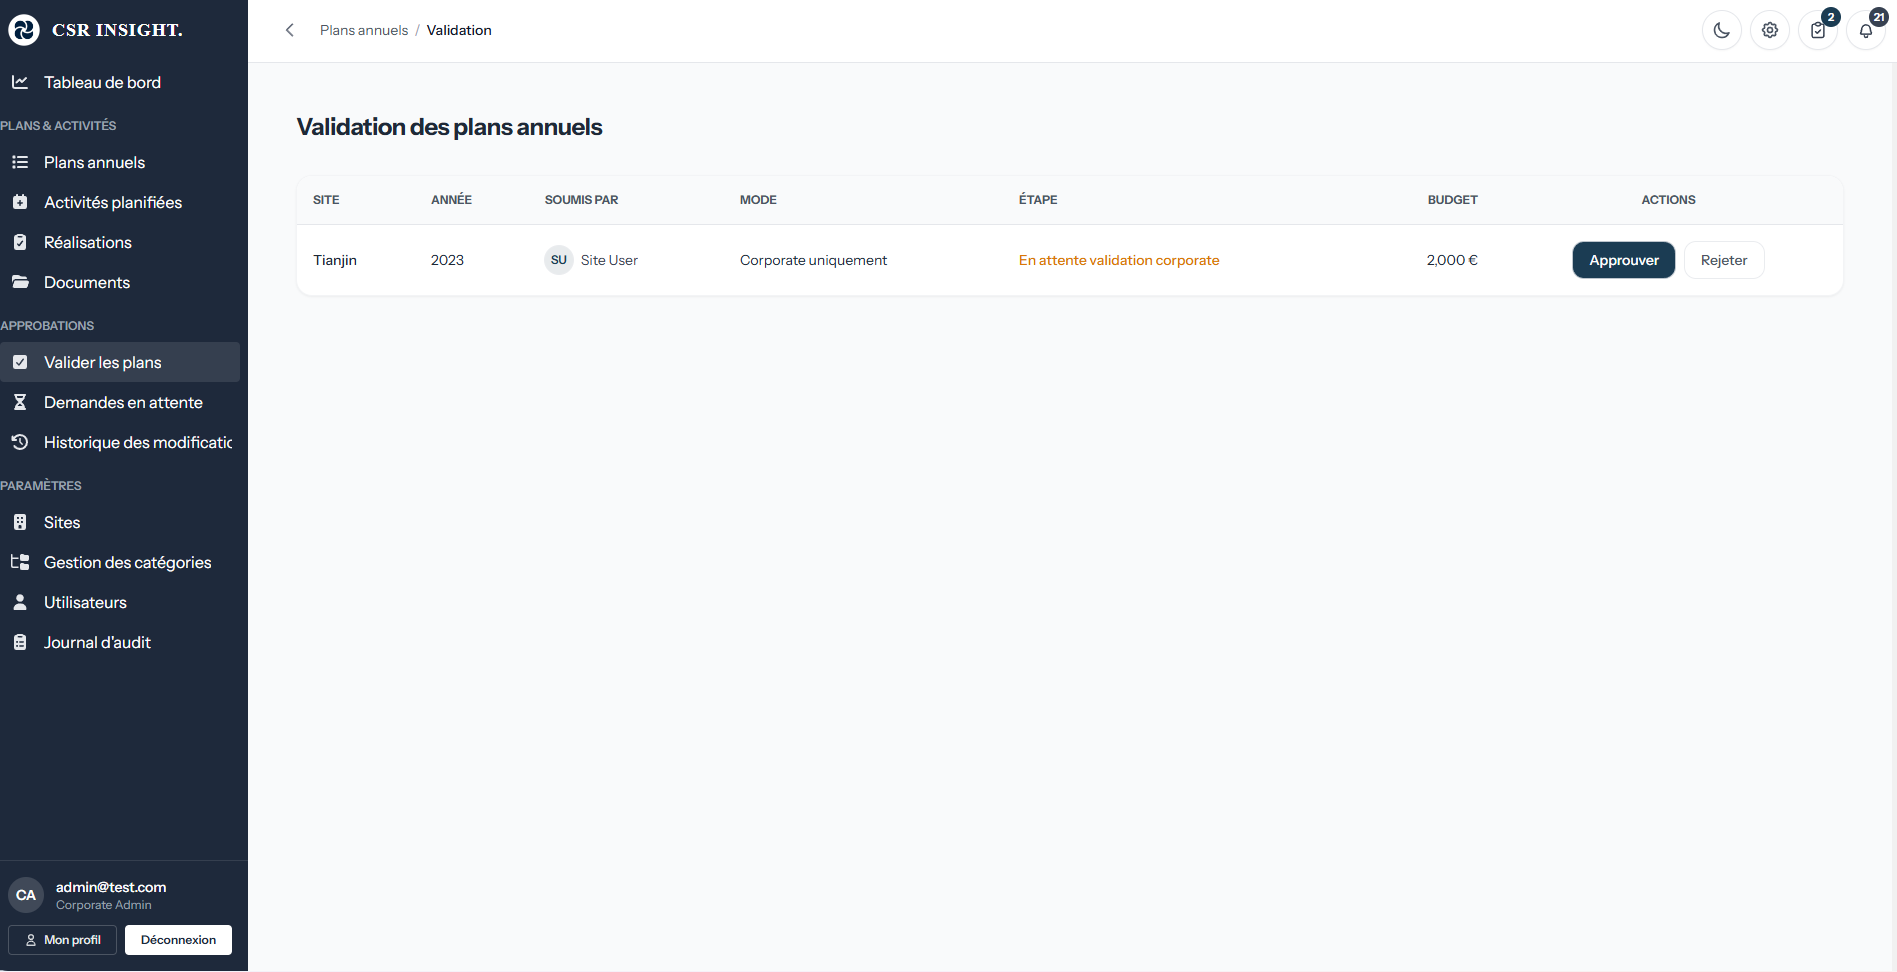
\includegraphics[width=0.92\linewidth]{figures/chapitre-05/realisation-interface-rejet-plan.png}
  \caption{Interface de rejet d'un plan.}
  \label{fig:ch5-realisation-rejet-plan}
\end{figure}%
}{%
\begin{figure}[H]
  \centering
  \fbox{\parbox{0.92\linewidth}{\centering\vspace{3.2cm}\textit{(Figure à insérer : \texttt{figures/chapitre-05/realisation-interface-rejet-plan.png})}\vspace{3.2cm}}}
  \caption{Interface de rejet d'un plan.}
  \label{fig:ch5-realisation-rejet-plan}
\end{figure}%
}

Cette interface illustre la fenêtre de rejet d'un plan, affichée lors de l'activation de l'action correspondante.
Elle permet à l'utilisateur Corporate de renseigner un motif de rejet, champ obligatoire garantissant la justification de la décision.
Elle offre également la possibilité de préciser, de manière optionnelle, les activités nécessitant des corrections.

L'objectif de cette interface est d'assurer un retour structuré et exploitable vers l'utilisateur à l'origine du plan, en encadrant le processus de correction.
Elle contribue également à renforcer la traçabilité des décisions prises, en conservant une justification claire associée à chaque rejet, tout en maintenant la cohérence du workflow global.

\subsection{Interface de demande de modification d'une activité}

La figure~\ref{fig:ch5-realisation-demande-modif-activite} présente l'interface de demande de modification d'une activité.

\IfFileExists{figures/chapitre-05/realisation-interface-demande-modification-activite.png}{%
\begin{figure}[H]
  \centering
  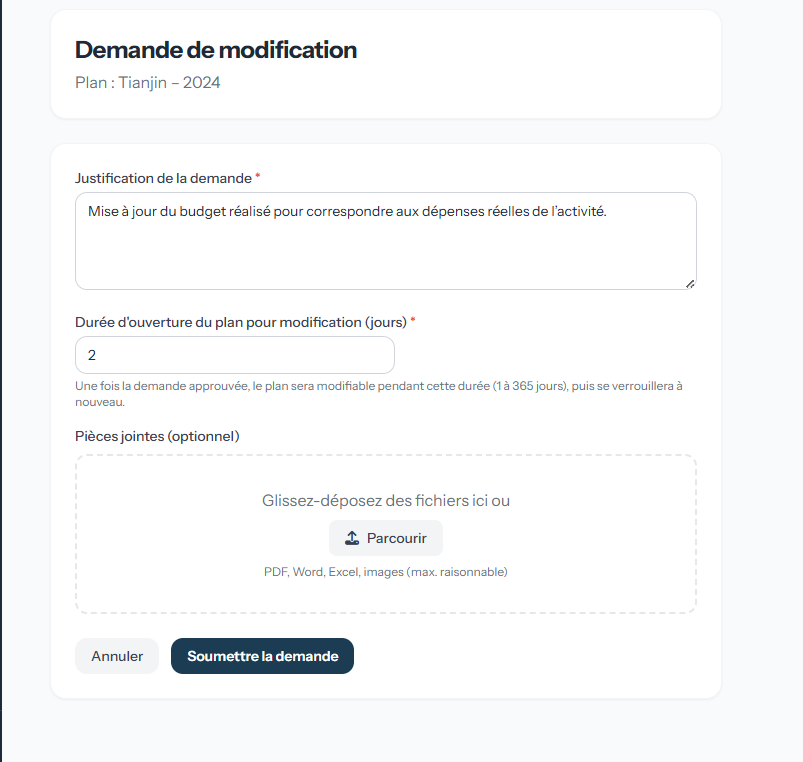
\includegraphics[width=0.92\linewidth]{figures/chapitre-05/realisation-interface-demande-modification-activite.png}
  \caption{Interface de demande de modification d'une activité.}
  \label{fig:ch5-realisation-demande-modif-activite}
\end{figure}%
}{%
\begin{figure}[H]
  \centering
  \fbox{\parbox{0.92\linewidth}{\centering\vspace{3.2cm}\textit{(Figure à insérer : \texttt{figures/chapitre-05/realisation-interface-demande-modification-activite.png})}\vspace{3.2cm}}}
  \caption{Interface de demande de modification d'une activité.}
  \label{fig:ch5-realisation-demande-modif-activite}
\end{figure}%
}

Cette interface présente la soumission d'une demande de modification d'une activité, permettant à l'utilisateur Site d'intervenir sur une activité déjà validée.
Elle se présente sous forme d'un formulaire structuré facilitant la saisie des informations nécessaires à l'analyse de la demande.

L'utilisateur doit renseigner une justification détaillée expliquant les raisons de la modification.
Il définit également une durée d'ouverture durant laquelle l'activité pourra être temporairement modifiée après approbation.
Une section spécifique permet d'ajouter des pièces jointes afin d'appuyer la demande avec des éléments justificatifs pertinents.

L'interface intègre des contrôles de validation pour garantir la complétude des informations avant la soumission.
Une fois envoyée, la demande est enregistrée et transmise à l'utilisateur Corporate pour traitement.
Elle s'inscrit ainsi dans un processus de contrôle post-validation, permettant de corriger les données tout en assurant la traçabilité et la cohérence du système.

\subsection{Interface du journal d'audit}

La figure~\ref{fig:ch5-realisation-journal-audit} présente l'interface du journal d'audit.

\IfFileExists{figures/chapitre-05/realisation-interface-journal-audit.png}{%
\begin{figure}[H]
  \centering
  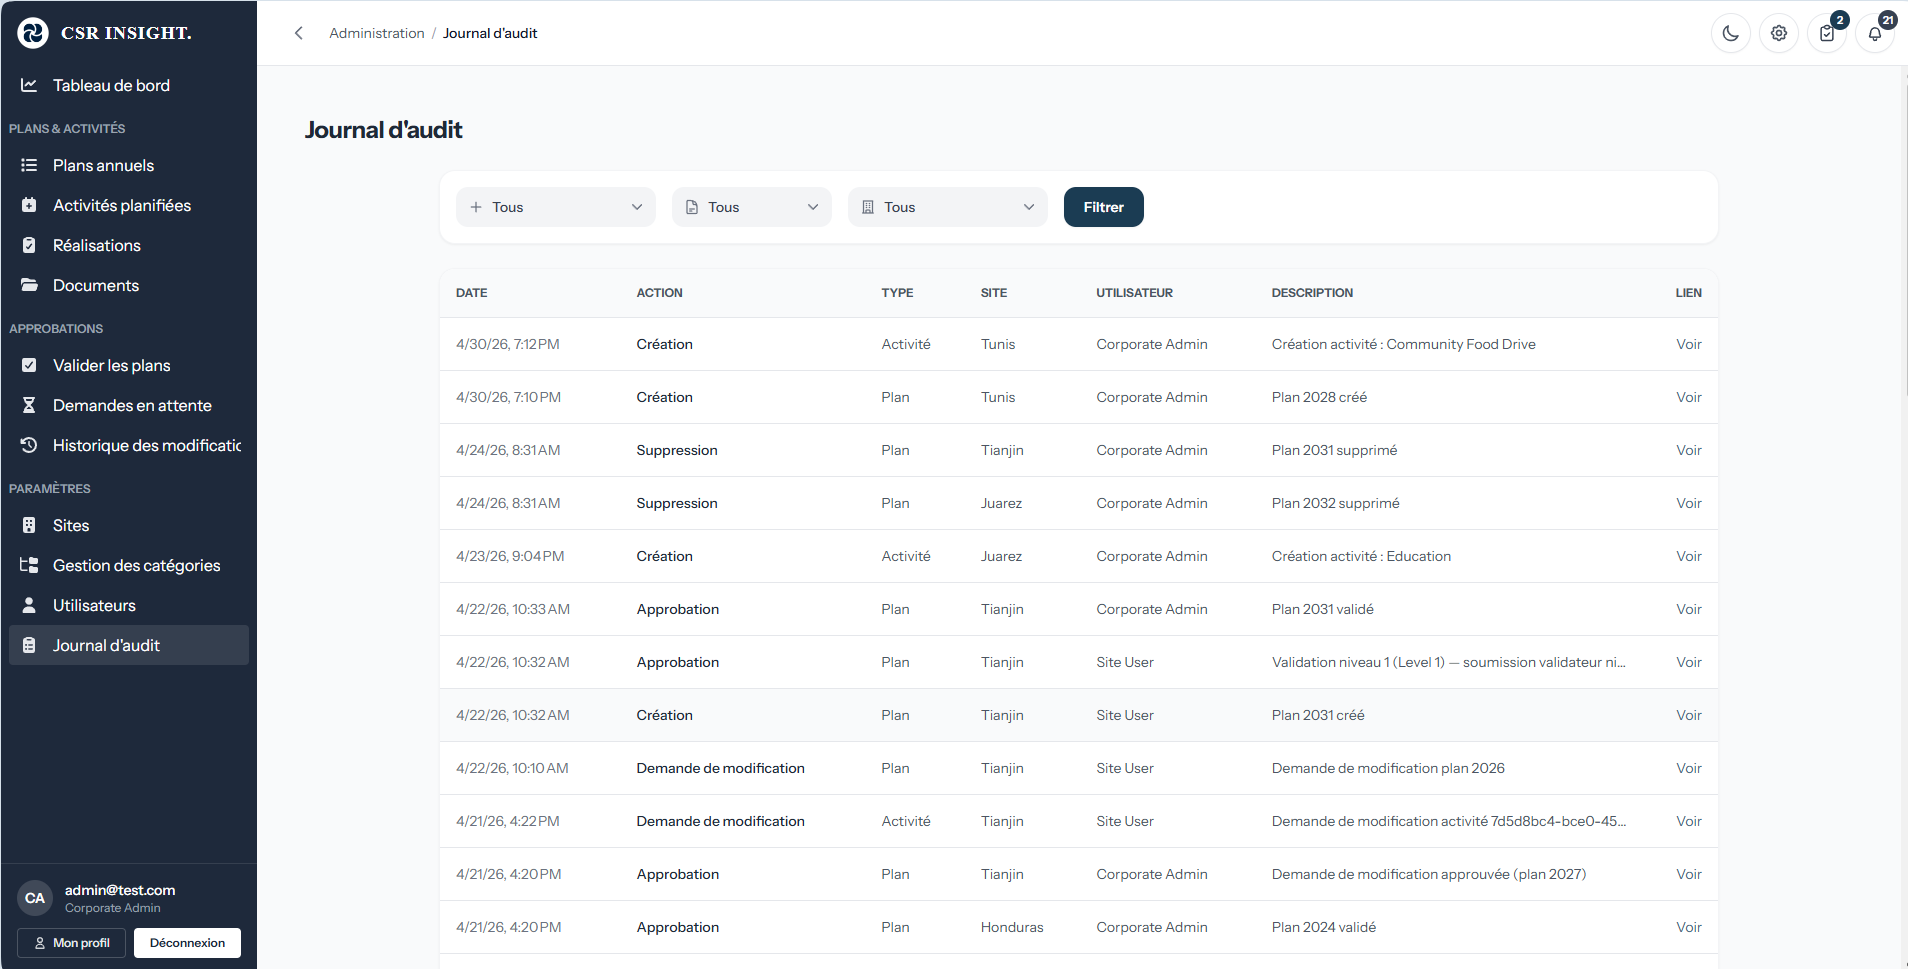
\includegraphics[width=0.92\linewidth]{figures/chapitre-05/realisation-interface-journal-audit.png}
  \caption{Interface du journal d'audit.}
  \label{fig:ch5-realisation-journal-audit}
\end{figure}%
}{%
\begin{figure}[H]
  \centering
  \fbox{\parbox{0.92\linewidth}{\centering\vspace{3.2cm}\textit{(Figure à insérer : \texttt{figures/chapitre-05/realisation-interface-journal-audit.png})}\vspace{3.2cm}}}
  \caption{Interface du journal d'audit.}
  \label{fig:ch5-realisation-journal-audit}
\end{figure}%
}

L'interface du journal d'audit est conçue pour assurer le suivi et la traçabilité de l'ensemble des actions effectuées sur la plateforme.
Ce module est accessible uniquement aux utilisateurs Corporate, afin de garantir un contrôle centralisé et sécurisé des opérations réalisées sur le système.

Elle offre une vue structurée sous forme de tableau chronologique regroupant les événements liés aux différentes entités, notamment les plans et les activités.
Chaque enregistrement détaille des informations clés telles que la date et l'heure de l'action, son type (création, validation, suppression, demande de modification, etc.), l'entité concernée, le site associé ainsi que l'utilisateur à l'origine de l'opération.
Une description explicite permet de comprendre rapidement le contexte de chaque action, avec la possibilité d'accéder directement à l'élément concerné.

Des options de filtrage sont également disponibles pour affiner l'affichage selon plusieurs critères, facilitant ainsi la recherche et l'analyse des opérations.
Cette interface constitue un élément essentiel du système, en assurant la transparence, la traçabilité et le suivi rigoureux de toutes les actions dans le cadre du workflow global.

\section{Tests et validation}

Les tests occupent une place centrale dans la méthodologie agile, car ils garantissent la qualité ainsi que la fiabilité des fonctionnalités développées. Avant le lancement d'un nouveau sprint, il est indispensable de valider les incréments prioritaires afin de vérifier leur bon fonctionnement et leur conformité aux besoins des parties prenantes.

\subsection{Test}

Dans cette partie, nous présentons une validation fonctionnelle consolidée des fonctionnalités du sprint~3 : validation et rejet des plans CSR, demandes de modification (plan), notifications, tâches et consultation du journal d'audit.
Le tableau~\ref{tab:ch5-scenarios-tests} synthétise les cas de test correspondants.

% Scénarios de test consolidés — chapitre 5 (workflow transverse)
\small
\PFETableSetup
\setlength{\LTpre}{0pt}
\setlength{\LTpost}{0pt}
\setlength{\LTleft}{\fill}
\setlength{\LTright}{\fill}
\setlength{\tabcolsep}{3.5pt}
\renewcommand{\arraystretch}{1.25}

\begin{longtable}{|>{\centering\arraybackslash}m{2.8cm}|
>{\raggedright\arraybackslash}p{2.5cm}|
>{\raggedright\arraybackslash}p{3.8cm}|
>{\raggedright\arraybackslash}p{4.3cm}|
>{\centering\arraybackslash}p{1.1cm}|}
\caption{Synthèse des cas de test du sprint 3}\label{tab:ch5-scenarios-tests}\\
\hline
\tableHeaderStyle
\multicolumn{1}{|c|}{\tableHeaderCell{Nom du cas d'utilisation}} &
\multicolumn{1}{c|}{\tableHeaderCell{Cas de test}} &
\multicolumn{1}{c|}{\tableHeaderCell{Description du cas}} &
\multicolumn{1}{c|}{\tableHeaderCell{Résultat attendu}} &
\multicolumn{1}{c|}{\tableHeaderCell{Résultat réel}} \\
\hline
\endfirsthead
\hline
\multicolumn{5}{|c|}{\tablename\ \thetable{} --- \textit{(suite)}} \\
\hline
\tableHeaderStyle
\multicolumn{1}{|c|}{\tableHeaderCell{Nom du cas d'utilisation}} &
\multicolumn{1}{c|}{\tableHeaderCell{Cas de test}} &
\multicolumn{1}{c|}{\tableHeaderCell{Description du cas}} &
\multicolumn{1}{c|}{\tableHeaderCell{Résultat attendu}} &
\multicolumn{1}{c|}{\tableHeaderCell{Résultat réel}} \\
\hline
\endhead
\hline
\multicolumn{5}{|r|}{\textit{Suite page suivante\ldots}} \\
\hline
\endfoot
\hline
\endlastfoot

\needspace{18\baselineskip}
\multirow{3}{=}{\centering Valider un plan CSR} &
Validation corporate (mode direct) &
Un utilisateur Corporate valide un plan soumis lorsque le mode le permet sans étape site préalable. &
Le plan passe au statut validé et n'est plus modifiable. &
Vrai \\
\cline{2-5}
 &
Validation en deux étapes &
Le Corporate tente de valider avant la validation du site lorsque le mode l'exige. &
Le système refuse et indique que la validation du site est requise en premier. &
Vrai \\
\cline{2-5}
 &
Consultation liste des plans soumis &
Ouverture de l'interface listant les plans en attente de décision. &
Les informations essentielles (site, année, statut, budget) sont affichées. &
Vrai \\
\hline

\needspace{12\baselineskip}
\multirow{2}{=}{\centering Rejeter un plan CSR} &
Motif obligatoire manquant &
Tentative de rejet sans saisir le motif de rejet. &
La soumission est refusée et le champ motif est signalé comme obligatoire. &
Vrai \\
\cline{2-5}
 &
Rejet avec motif valide &
Saisie d'un motif de rejet et confirmation du rejet. &
Le plan est rejeté, le statut est mis à jour et le motif est conservé. &
Vrai \\
\hline

\needspace{18\baselineskip}
\multirow{3}{=}{\centering Soumettre une demande\\de modification pour un plan} &
Données incomplètes &
Soumission d'une demande sans justification ou sans durée d'ouverture requise. &
Message d'erreur listant les champs à compléter. &
Vrai \\
\cline{2-5}
 &
Pièce jointe non conforme &
Ajout d'un fichier de type ou taille non autorisé. &
Le fichier est refusé avec un message explicite. &
Vrai \\
\cline{2-5}
 &
Soumission valide &
Demande complète sur un plan verrouillé avec justification et durée. &
La demande est enregistrée avec le statut « en attente » et associée au plan. &
Vrai \\
\hline

\needspace{12\baselineskip}
\multirow{2}{=}{\centering Traiter une demande\\de modification} &
Approbation corporate &
Examen puis approbation d'une demande en attente. &
Le statut de la demande est mis à jour et le site est notifié. &
Vrai \\
\cline{2-5}
 &
Rejet avec justification &
Rejet d'une demande avec commentaire obligatoire. &
Le statut est mis à jour et le motif est conservé pour le site. &
Vrai \\
\hline

\needspace{12\baselineskip}
\multirow{2}{=}{\centering Recevoir des\\notifications} &
Notification après validation &
Un événement de validation génère une notification pour les acteurs concernés. &
La notification apparaît dans le centre de notifications. &
Vrai \\
\cline{2-5}
 &
Marquer comme lue &
L'utilisateur ouvre ou marque une notification comme lue. &
L'état de lecture est mis à jour et le compteur reflète le changement. &
Vrai \\
\hline

\needspace{12\baselineskip}
\multirow{2}{=}{\centering Gérer les tâches} &
Tâche créée après un événement &
Soumission ou validation déclenchant la création d'une tâche assignée. &
La tâche apparaît dans la liste des tâches de l'utilisateur concerné. &
Vrai \\
\cline{2-5}
 &
Ouverture d'une tâche &
Clic sur une tâche pour accéder au contexte (plan ou demande). &
La navigation mène à l'écran attendu. &
Vrai \\
\hline

\needspace{12\baselineskip}
\multirow{2}{=}{\centering Consulter le\\journal d'audit} &
Affichage chronologique &
Consultation de la liste des événements par un profil Corporate autorisé. &
Les actions sont listées avec date, type, entité et auteur. &
Vrai \\
\cline{2-5}
 &
Filtrage par critères &
Application de filtres (site, type d'action, période). &
La liste se restreint aux enregistrements correspondants. &
Vrai \\
\hline

\end{longtable}
\normalsize


\newpage

Les flux liés aux demandes de modification, aux notifications et aux tâches ont également été vérifiés avec \emph{Postman}, en contrôlant les réponses après enchaînement des actions corporate.
Les figures~\ref{fig:ch5-postman-cr},~\ref{fig:ch5-postman-notif} et~\ref{fig:ch5-postman-tasks} illustrent des exemples de ces vérifications.

\IfFileExists{figures/chapitre-05/postman-change-requests.png}{%
\begin{figure}[H]
  \centering
  \includegraphics[width=0.92\linewidth]{figures/chapitre-05/postman-change-requests.png}
  \caption{Tests Postman : demandes de modification.}
  \label{fig:ch5-postman-cr}
\end{figure}%
}{%
\begin{figure}[H]
  \centering
  \fbox{\parbox{0.92\linewidth}{\centering\vspace{3.2cm}\textit{(Figure à insérer : \texttt{figures/chapitre-05/postman-change-requests.png})}\vspace{3.2cm}}}
  \caption{Tests Postman : demandes de modification.}
  \label{fig:ch5-postman-cr}
\end{figure}%
}

\IfFileExists{figures/chapitre-05/postman-notifications.png}{%
\begin{figure}[H]
  \centering
  \includegraphics[width=0.92\linewidth]{figures/chapitre-05/postman-notifications.png}
  \caption{Tests Postman : notifications.}
  \label{fig:ch5-postman-notif}
\end{figure}%
}{%
\begin{figure}[H]
  \centering
  \fbox{\parbox{0.92\linewidth}{\centering\vspace{3.2cm}\textit{(Figure à insérer : \texttt{figures/chapitre-05/postman-notifications.png})}\vspace{3.2cm}}}
  \caption{Tests Postman : notifications.}
  \label{fig:ch5-postman-notif}
\end{figure}%
}

\IfFileExists{figures/chapitre-05/postman-tasks.png}{%
\begin{figure}[H]
  \centering
  \includegraphics[width=0.92\linewidth]{figures/chapitre-05/postman-tasks.png}
  \caption{Tests Postman : tâches.}
  \label{fig:ch5-postman-tasks}
\end{figure}%
}{%
\begin{figure}[H]
  \centering
  \fbox{\parbox{0.92\linewidth}{\centering\vspace{3.2cm}\textit{(Figure à insérer : \texttt{figures/chapitre-05/postman-tasks.png})}\vspace{3.2cm}}}
  \caption{Tests Postman : tâches.}
  \label{fig:ch5-postman-tasks}
\end{figure}%
}

\subsection{Validation}

Une revue de fin de sprint avec le \emph{Scrum Master} et le \emph{Product Owner} a permis de valider les parcours du sprint 3 : Gestion transverse des validations, notifications et traçabilité (validation et rejet de plans, demandes de modification, notifications, tâches et journal d'audit). Les correctifs portent notamment sur les messages utilisateur, la cohérence des statuts entre demandes et entités concernées, ainsi que sur le rafraîchissement des listes après action corporate.

\section{Conclusion}

Ce sprint renforce la gouvernance des données CSR en introduisant un mécanisme de gestion globale:
contrôle des validations, traitement des demandes de modification, notifications, tâches et audit.

Le chapitre suivant présente le sprint \emph{BI \& KPI} (tableaux de bord, intégration Power BI et indicateurs de pilotage).
